\documentclass[10pt,draftclsnofoot,onecolumn,journal,compsoc]{IEEEtran}

\usepackage[margin=0.75in]{geometry}
\usepackage{graphicx}
\usepackage{caption}
\usepackage{hyperref}
\usepackage{enumerate}
\usepackage{pgfgantt}
\usepackage{tabu}
\usepackage[english]{babel}\usepackage[numbers]{natbib}
\usepackage{natbib}


\renewcommand{\bibsection}{}

\renewcommand{\linespread}{1.0}
\title{Prototype Big Data Archive in a Public Cloud}
\author{
  \IEEEauthorblockN{Group 56: Pathfinder of Big Data\\Zhi Jiang, Isaac T Chan, Zhaoheng Wang} \\
  \IEEEauthorblockA{CS 461: Senior Capstone Fall 2016 \\ Oregon State University}
}
\date{}

\IEEEtitleabstractindextext{
	\begin{abstract}
	OSU campuses generate data constantly from multiples sources, including computer labs, wireless usage, student devices, and many others. This quantity of data, also known as big data, can effectively represent all kinds of behaviors of students for information technology. For example, analysis can be run to determine common student behaviors in order to allocate OSU resources more effectively. Currently, the data is very difficult to manage because it is collected from multiple sources and is impossible to analyze. The data is neither stored in the same formats nor in the same locations, meaning it is inaccessible and useful information is unable to be extracted.Our goal for this project is to unify and organize the data onto the consistent cloud platform of Amazon Web Services, which additionally provides utilities to manage and analyze. To achieve this, we plan to have a working prototype at the Engineering Expo that demonstrates the value of analyzing OSU big data and how the cost-to-value of our Amazon cloud solution compares to locally-hosted hardware. Our prototype will allow OSU big data to be analyzed and eventually it can be scaled to analyze all the data that OSU collects.
	\end{abstract}
}


\begin{document}
% cover page    
    \maketitle
    \IEEEdisplaynontitleabstractindextext
    \IEEEpeerreviewmaketitle

    \newpage
% catalog    
    \tableofcontents

    \newpage
% content    
    \section{Introduction}
        \subsection{Purpose}
        The purpose of this requirements document is to address specification for our product. We will clearly explain functionality, performance, attributes and design constraints of our product while remaining at a high-level to avoid technical details.The intended audience of this document is the client, our development group, and assessors of our work. Our group and client must share a mutual understanding of the project and all the details it entails, to confirm that our final product meets and matches all expectations. Assessors of our work may reference this document to compare it to our final product, again to ensure our final product matches requirements.
        
        \subsection{Scope}
        The name of this product is “Prototype Big Data Archive in a Public Cloud”, and will be used to to implement all operations about data from multiple sources and ensure data can be unified and organized onto a consistent cloud platform. The product can mine valuable information from data to integrate them because the data can reflect behaviors of students and staffs.\\
        
        \noindent A huge amount of data is generated when students and staffs use various information technologies such as printers and computers. The product will provide a database which can systematically deal with the data, so it contains several functions about operation for data such as ingest, store, manage and retrieve. On the other hand, the product is also able complete basic reporting and analysis. Therefore, these functions of product can help OSU Information Services staffs conveniently manage data, and they can directly and expediently understand behaviors of students and staffs according to analysis.

        \subsection{Definitions, acronyms, and abbreviations} 
        \begin{tabu} to \hsize {|X|X[2,l]|}
        \hline
        \textbf{Term} & \textbf{Definition}\\
        \hline
        User & The person who interact with our project \\
        \hline
        Big data & A holistic information management strategy that is used to integrate and management a large set of new types of data alongside traditional data. applications\cite{big data}\\
        \hline
        Cloud platform & The cloud platform is using the cloud computing technology.So in the cloud computing, Platform as a Service(PaaS) is used to integrate cloud-based computing environment such as running and development of applications. On the other hand, Infrastructure as a Service(IaaS) is used provide basic resources like operating systems and storage\cite{cplatform}\\
        \hline
        AWS & Amazon web service, a Platform as a service(PaaS) offered by Amazon \\
        \hline
        DB & Database\\
        \hline
        Nosql & non-relational database\\
        \hline
        \end{tabu}
        
        \subsection{References}
        
        \begin{thebibliography}{9}
    
        \bibitem{IEEE}\textit{IEEE Recommended Practice for Software Requirements Specifications}, The Institute of Electrical and Electronics Engineers, Inc., New York, NY, 1998.
        \bibitem{big data}"What is Big Data?", \textit{Oracle.com}, 2016. [Online]. Available: https://www.oracle.com/big-data/index.html. [Accessed: 11- Nov- 2016].
        \bibitem{cplatform}"What Is Platform as a Service (PaaS) in Cloud Computing?", \textit{dummies}, 2016. [Online]. Available: http://www.dummies.com/programming/cloud-computing/hybrid-cloud/what-is-platform-as-a-service-paas-in-cloud-computing/. [Accessed: 11- Nov- 2016].
        \bibitem{AWS Rate}"AWS Rates Highest on Cloud Reliability", \textit{EnterpriseTech}, 2016. [Online]. Available: http://www.enterprisetech.com/2015/01/06/aws-rates-highest-cloud-reliability/. [Accessed: 08- Nov- 2016].
        \bibitem{Cloud}"Advantages and Disadvantages of Cloud Computing", \textit{LevelCloud}, 2016. [Online]. Available: http://www.levelcloud.net/why-levelcloud/cloud-education-center/advantages-and-disadvantages-of-cloud-computing/. [Accessed: 08- Nov- 2016].
        
        \end{thebibliography}

        \subsection{Overview}
        Following this introduction is a section describing the product as a whole. This includes perspective, function, user characteristics, constraints, and assumptions/dependencies. The purpose of the section is to provide in-depth details on requirements of the product. Finally, this document is concluded with a section on specific requirements.
   
    \newpage
    
    \section{Overall description}
        \subsection{Product perspective}
        In terms of perspective, our product is the most important part of a larger system. The larger system includes three parts, and which are collecting data, managing data and analysing data, so main functionality of the product are used to manage data. The produce is independent of other parts of whole system because client will provide sample of data to test this product, thus there is no interconnection between our product and collecting data part. On the other hand, we need to complete basic reporting and analysing function. Hence there should be data transmission between database and data analytics.
        \begin{figure}[h]
        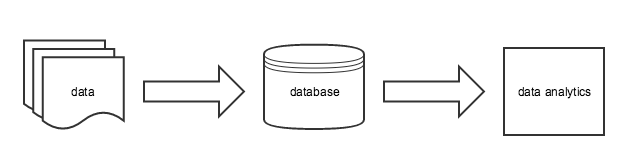
\includegraphics[width=15cm, height=4cm]{project.png}
        \centering
        \caption{work flow of entire system}
        \end{figure}
        
       \subsection{Hardware Interface} 
       The database is built on public cloud so AWS platform will provide all aspects of the hardware supports. For example, high capacity solid state disks will used to store data items as a storage of product. And low-latency network connection can ensure maximum speed of accessing database.

        \subsection{Software interface}
        The AWS platform contains a variety of software provisioning for our product. On the one hand, developers can use proper programming language to implement functions of product base on via SDKs provided by AWS. On the other hand, the management console can help developer monitor all kinds of condition of database such as calculating throughput and cost. 
       
       \subsection{Production function}
       The product will store different types of data such as log file, clickstream data in database. Besides, the product will provide enough space to hold vast amount of data, and it is able to build index and process data in batch. Furthermore, the database will implement some basic operations including inserting, deleting, updating and searching for data. Eventually, analysis technical will communicate to database, and then data will be accessed quickly by analysis technical while all of valuable data will be used to represent behaviors of students and staffs.

        \subsection{User characteristics}
        There is only one type of user that interact with our product: data analyzer. Staff who analyze the data can insert different types of data into database. Then, they could search the information base on the specific condition. After searching, data analyzer could do some management for the data such as sorting data. Finally, data analyzer could also extract the data from database and load it into a data analysis tool to do the analysis. 

        \subsection{Constraints}
        In implementation, there are minimal constraints placed on design. There are, however, certain aspects of development that we must keep in mind, including resource limits, implementation language, and development environment. The main aspect being that development on the AWS platform will cost our client money. AWS charges for computing time, temporary data storage, and database usage. Though it is unlikely that we will run into any upper budget limit, we need to have in mind the charges in order to eliminate resource waste. Amazon also offers a budget tool for our client to track our budget usage. It can also provide a forecast for future budget, so we can know in advance if we are approaching any limit. In terms of implementation language, AWS is flexible in the choice of coding language; we are free to choose any programming language that they support. Finally, our development will be done from our personal machines; as a cloud computing service, Amazon’s resources can be freely accessed by us wherever on any operating system.

        \subsection{Assumptions and dependencies}
        Because the nature of the project is to produce a prototype of a cloud-based big data archive, there is an assumption that our final product will be a competitive solution for OSU’s data analytics, compared to a locally-hosted solution. From this base-assumption, there are several dependencies to keep in mind, including scalability, future maintenance, and security.\\ 
        
        \noindent Our development will be done mostly with small test-sets of data, with student information anonymized before given to us. Therefore, a large concern is scalability - our solution must be able to work with potentially enormous data sets in a reasonable time. Database retrieval time is critical; the solution is almost useless if it takes an inappropriately long time to extract data from our implemented database. Additionally, database manipulation time, such as “joins” is an important factor when considering adopting the final product. Other metrics will be determined as we begin design implementation.

	\newpage
    
    \section{Specific requirements}
        \subsection{Functional requirements}
        \begin{itemize}
        \item The user can insert any types of data they want into database.\\
        Description: In this function, the user should be able to insert multiple data types in database such as log file and click stream. These data could be non-relational.\\
        Sequence of operations: 1) access the management console of database. 2) upload data to management console 3) use inserting function to store data in database 4) output result of inserting data.\\
        Test: When inserting different types of data in database, there should not exist any error about inserting. On the other hand, we can do random testing to randomly choose a set of data and then check diversity of them.
        \\
        \item The user can find information in database.\\
        Description: In this function, the user should be able to find information in database.\\
        Sequence of operations: 1) access the management console of database. 2) enter information which needs to be searched. 3) use searching function to search information in database 4) output related data items.\\ 
        Test: We can use unit testing to check correctness of results after we find a item.
        \\
        \item The user can do conditional find for information.\\
        Description: In this function, the user should be able to search information according some specific condition. For example, user can set some restrictions like they can only find data about senior students or engineering students.\\
        Sequence of operations: 1) access the management console of database. 2) enter information which needs to be search and set specific condition. 3) use search function to search information bases on condition. 4) output related data items.\\
        Test: We can create specific unit testing according to finding condition. Then to use these unit testings to check correctness of results when we conditionally search an item.
        \\
        \item The user can aggregate data and then find specific result.\\
        Description: In this functions, the user should be able to use aggregate methods to find some specific results such as average of GAP or the highest utilization ratio of certain printer on the campus.\\
        Sequence of operations: 1) access the management console of database. 2) enter result which needs to be aggregated. 3) use aggregation function to specific result. 4) output specific results.\\
        Test: We can use unit testing to check correctness of results after aggregate data. But we need to do some extra computing by ourselves for those specific results like average of GAP.
        \\
        \item The user can sort some specific data.\\
        Description: In this function, the user should be able to sort specified data. For example, user can sort amount of credits for all engineering students.\\
        Sequence of operations: 1) access the management console of database. 2) target a set of data which need to be sorted. 3) use sort function to sort a set of data. 4) output sorted list of data.\\
        Testing: When database return sorted list, we can use unit testing to traversal the entire list and check correctness of relationship between adjacent items.
        \end{itemize}

        \subsection{Performance requirements}
        Performance metrics will be determined and assessed as we begin implementation. Currently there is no reliable basis of comparison for any performance metrics regarding database operations, such as data insertion, manipulation, and searching. A basis of performance comparison is subjective and may not fit our implementation exactly, thus are not defined at this point. Performance times for operations can be assessed by the client for acceptable runtimes and after client response, operating methods may be altered.
        
        \subsection{Software system attributes}
        Reliability:\\
        Compared to a locally hosted solution, a cloud platform offers additional benefits regarding reliability. When it comes to server maintenance, updates, and upgrades, downtime is a concern. Server downtime can interrupt analysis database access. Cloud platforms provide a reliable software system with minimal downtime\cite{AWS Rate}. There are agreements and certifications required by cloud providers\cite{Cloud} for acceptable amounts of downtime. As we implement our big data prototype with a cloud platform, reliability requirements are fulfilled by the cloud platform.\\
        \\
        Availability:\\
        Additionally, cloud platforms provide a method of access from anywhere, only requiring user credentials and an Internet connection. This is another benefit to the cloud solution.\\
        \\
        Security:\\
        Security is an important attribute. Our development will be using test-sets of user anonymized data, which protects us from liability and knowledge of specific users. Also, databases do have vulnerabilities, like any other software. We will consider prevention of malicious interactions, such as injection attacks. On the same note, if for any reason the database were to go down, we may want to have implemented a backup database. This will depend on the transfer time and quantity of data to store; if it is easily uploaded there is no reason to require a backup database.\\
        \\
        Maintainability:\\
        Future maintenance is another concern. Our implementation will be maintained by others of varying levels of expertise. Therefore, our product must have readable code and abundant, clear documentation.
    
    \newpage
    \section{Schedule} 
        \begin{ganttchart}[vgrid, hgrid]{1}{22}
        \gantttitle{Fall}{4}
        \gantttitle{Winter}{10}
        \gantttitle{Spring}{8}\\
        
        \gantttitlelist{7, 8, 9, 10}{1}
        \gantttitlelist{1,...,10}{1}
        \gantttitlelist{1,...,8}{1}\\
        
        \ganttbar{Technology Review}{1}{1} \\
        \ganttbar{Design Plan}{2}{4} \\
        
        \ganttbar{Database Table Implementation}{5}{5} \\
        \ganttbar{Data loading for checking table}{6}{7}\\
        \ganttbar{Implement insert, sort and search}{8}{9}\\
        \ganttbar{Implement aggregation}{10}{12}\\ 
        \ganttbar{Data visualization}{13}{14} \\
        
        \ganttbar{Test for functionality}{15}{16} \\
        \ganttbar{Performance Optimization}{17}{18}\\
        \ganttbar{Security Optimization}{19}{20}\\
        \ganttbar{Cost Comparison}{21}{22}
        \end{ganttchart}



    \newpage
        \thispagestyle{empty}
        \noindent\begin{tabular}{ll}
        \makebox[2.5in]{\hrulefill} & \makebox[2.5in]{\hrulefill}\\
        Client & Date\\[8ex]% adds space between the two sets of signatures
        \makebox[2.5in]{\hrulefill}\\
        Developer 1\\[8ex]
        \makebox[2.5in]{\hrulefill}\\
        Developer 2\\[8ex]
        \makebox[2.5in]{\hrulefill}\\
        Developer 3\\[8ex]
        \end{tabular}

\end{document}

